\documentclass{article}
\usepackage{iclr2027_conference,times}
\usepackage{amsmath}
\usepackage{amssymb}
\usepackage{booktabs}
\usepackage{graphicx}
\usepackage{hyperref}

\title{Acting Through a Behavior Flow: Restricted Action Interfaces and Their Ceiling}

\author{Anonymous}

\begin{document}
\maketitle

\begin{abstract}
We are testing whether zero-shot offline RL can avoid off-support action optimization by acting entirely through a frozen behavior flow. The approach works partially: LatentFlowPSM reaches $0.236$ success on cube-single-play versus $0.068$ for the behavior flow alone, but then saturates near $0.22$. A per-task RL control in the same latent action space reaches the same ceiling, suggesting that the bottleneck is not specific to successor-measure learning. Decoder diagnostics provide a likely explanation: sampled latent actions recover only $42\%$ of local dataset action dispersion and remain separated from the actions selected by a strong per-task policy---which themselves sit roughly $1.7\times$ farther from the local empirical actions than from our decoder, under candidate-count-matched minimum-distance statistics (the unmatched $3\times$ figure was inflated by comparing 512 decodes against 32 neighbors). Our current hypothesis is that the restriction has two layers: the learned behavior model covers only part of the local action variation present in the data, and a high-performing unconstrained policy appears to exploit actions that are not represented in the local empirical action cloud at all. The next experiment relaxes this interface with a bounded residual and directly measures the trade-off between decoder restriction and task performance.
\end{abstract}

\section{Setting}
A successor measure $M^\pi(s,a,X)$ gives the discounted occupancy of state sets $X$ under $\pi$ after $(s,a)$; once learned, it evaluates \emph{any} downstream reward by integration, which is the basis of zero-shot RL \citep{touati2021learning}. Offline RL's central failure mode is off-support actions: the critic is queried where the data says nothing, and the standard fix is a penalty that fights the actor.

Our starting idea was simple: instead of penalizing off-support actions, restrict RL to actions produced by a behavior model. We fit a behavior flow $G(s,u)$ mapping noise $u\sim\mathcal{N}(0,I)$ to dataset actions by flow matching (the BC-only flow of FQL; \citealp{park2025fql}), freeze it, and do all of RL in latent space: policies emit $u$, the executed action is the frozen decode $G(s,u)$. Every executed action is therefore an action the \emph{learned model} can produce. We flag the gap in that guarantee now because it becomes the main result later: the decoder restricts actions to those expressible by the learned behavior model, which is not the same as the dataset's true conditional support. Benchmarks are OGBench manipulation and navigation tasks \citep{park2024ogbench}.

\section{The pipeline}
Three stages; each stage's output is frozen before the next begins.

\begin{table}[h]
\centering
\small
\begin{tabular}{@{}llll@{}}
\toprule
Stage & What it does & Cost & Published? \\
\midrule
A. Behavior flow & Fit $G(s,u)$ by flow matching (FQL BC-only) & $\sim$1\,h & -- \\
B. Inversion & Per transition, find the latent $u^*$ decoding to the recorded action & 4--19\,h & yes \\
C. Latent PSM & Successor measure $\psi(s,w,u)$ over latents + amortized latent actor & $\sim$3\,h & -- \\
\bottomrule
\end{tabular}
\caption{The three-stage pipeline. Stage-B artifacts (per-transition preimage latents for every dataset) are public on Hugging Face (\texttt{amsks/psmflows-preimages}).}
\label{tab:pipeline}
\end{table}

Stage B solves, for each recorded transition $(s,a)$, the preimage problem
\begin{equation}
u^*(s,a) \;=\; \arg\max_{u}\; p(u)\,\,\text{s.t.}\;\; G(s,u)=a,
\label{eq:preimage}
\end{equation}
approximated by an EM posterior over latents ($\alpha=20$, $N=200$ particles). Quality checks: final-step mean effective sample size 94.6 (pointmaze) / 81.3 (cube); roundtrip error $\|G(s,u^*)-a\|\sim 10^{-4}$; recovered latents are typical, sitting inside the $\chi^2$ band for $\mathcal{N}(0,I)$.

\section{Finding 1: the failure is the index, not the measure}
\emph{The natural policy family ``fixed noise $=$ policy index,'' $\pi_u(s)=G(s,u)$, contains almost no goal-reaching behaviors, so GPI over this family was already at the best performance achievable within it.}

The mechanism starts with an observation about the data. In these datasets the goal is absent from the observation, so the action needed to follow the expert trajectory cannot be inferred from $s$ alone. It therefore has to be encoded in $u_t$, and the inferred $u_t$'s vary substantially from step to step. The two statistics say different things: within-episode preimage variance is $0.99\times$ the marginal variance, so individual episodes span nearly the full latent variability of the dataset; and the lag-1 autocorrelation of $u_t^*$ within episodes is $0.27$, decaying to roughly zero by lag 50, so what latent identity exists is also only weakly persistent over time. There is therefore little persistent episode-level structure in the inferred latents for a fixed $u$ to recover.

The reachability experiment tests the consequence directly (Figure~\ref{fig:reachability}). On pointmaze ($d_a=2$), a $13\times13$ grid of fixed latents covers the whole latent box: \textbf{0 of 233} latents ever reach the goal, with best closest-approach $1.32$ in a maze spanning $\sim$30 units. Cube: $2/128$ latent-episodes succeed ($\sim$1\%); antmaze: $5/64$ ($\sim$4\%). The family contains only two regimes: a typical $u$ orbits near the start (path length 164, net displacement 1.4), while a saturated $u$ marches in a constant heading. The observed fixed-$u$ GPI floor ($0.02$--$0.06$ on cube) matches the best performance achievable within this policy family---selection was already extracting everything the family contains.

The successor measure itself was not the bottleneck. The problem was the policy family it indexed: fixing one latent $u$ across an episode produced almost no goal-reaching behaviors, so GPI had no useful policies to select among.

\begin{figure}[t]
\centering
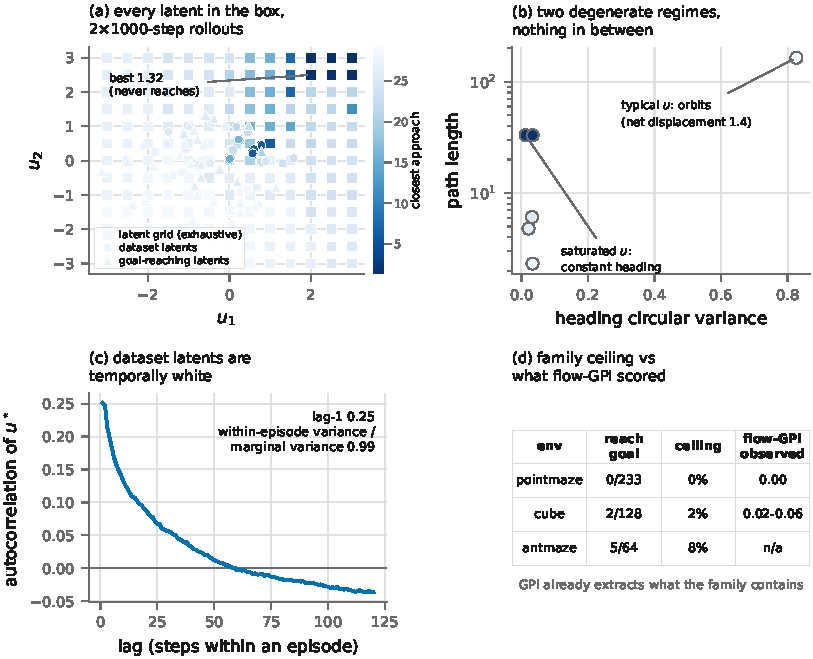
\includegraphics[width=0.9\linewidth]{figures/fig_reachability.pdf}
\caption{Exhaustive reachability of the fixed-$u$ family. On pointmaze a $13\times13$ latent grid covers the box; 0 of 233 fixed latents reach the goal (best closest-approach 1.32; maze span $\sim$30). Typical latents orbit near the start (path length 164, net displacement 1.4); saturated latents march in a constant heading. Cube: 2/128; antmaze: 5/64.}
\label{fig:reachability}
\end{figure}

\section{LatentFlowPSM}
The failed construction used $u$ for two jobs at once: it selected a policy and it determined the action executed at every state. LatentFlowPSM separates these roles. A task vector $w$ identifies the policy, while an amortized actor chooses a state-dependent latent action $u(s,w)$, which the frozen flow then decodes into an environment action. The successor feature head $\psi(s,w,u)$ over latent actions is trained with a TD backup that bootstraps the actor's own latent at the next state:
\begin{equation}
\psi(s,w,u) \;\leftarrow\; \phi(s') \;+\; \gamma\,\psi\!\big(s',\,w,\,u(s',w)\big).
\label{eq:backup}
\end{equation}
The actor is a noise-conditioned network with $\tanh$-bounded output, trained on a normalized value term $-Q/|Q|$ plus a behavior-cloning term. The cloning term exists for a specific reason: because unconstrained optimization over latent space can move the actor away from the latents observed during inversion, we regularize the actor toward the inferred dataset latents $u^*$. At evaluation, the task vector is the closed form $w=\mathbb{E}[r\,\phi(s')]$ over a reward-labeled sample. This is the standard successor-feature recipe \citep{touati2021learning}, transplanted into the flow's latent space.

\section{Finding 2: the ceiling is shared with per-task RL}
\emph{LatentFlowPSM improves substantially over every decoder-restricted control, then saturates near $0.22$---and per-task RL in the same latent space saturates at the same level.}

\begin{table}[h]
\centering
\small
\begin{tabular}{@{}lll@{}}
\toprule
Method & Success & Notes \\
\midrule
BC flow alone & 0.068\,[0.049, 0.094] & behavior-cloning floor \\
Fixed-$u$ flow-GPI & 0.02--0.06 & family limit (\S3) \\
Latent-GPI (same repr., actor-free) & 0.055 & \\
\textbf{LatentFlowPSM (ours)} & \textbf{0.236 $\pm$ 0.071} & \\
Bilinear PSM (peer) & 0.156\,[0.127, 0.190] & 1 of 3 seeds evaluated \\
FB (peer, action space) & 0.716 / 0.730 / 0.716 & unrestricted action space \\
FQL per-task topline & 0.949 $\pm$ 0.063 & not zero-shot \\
\bottomrule
\end{tabular}
\caption{Cube-single-play. 500-episode evals; intervals are Wilson 95\% for single runs and seed mean $\pm$ 95\% CI otherwise. LatentFlowPSM: 5 seeds (0.318/0.236/0.176/0.260/0.188); FB: 3 seeds; FQL: 3 seeds. Bilinear PSM is the peer method of \citet{agarwal2024protosm}.}
\label{tab:main}
\end{table}

On antmaze, LatentFlowPSM reaches 0.22/0.26/0.22 (3 seeds) vs.\ a BC control of 0.090---the same $\sim$2.5$\times$ pattern. On pointmaze both our method \emph{and} the action-space PSM control score 0.0: the goal is not in the observation, so the whole method family fails there. This is a framing point, not a defect of the latent construction.

The two unconstrained baselines contextualize the gap. FB at $\sim$0.72 shows there is enough information in the dataset and the representation-learning problem to obtain substantially better zero-shot behavior; the performance loss appears when optimization is restricted through the learned behavior decoder. FQL at $\sim$0.95 shows the task is solvable and the dataset supports much better behavior under a less restrictive interface. Importantly, FQL's actor receives the $Q$-gradient directly on its action output and is not constrained to outputs of the frozen decoder (its flow appears only in behavior-cloning and distillation terms), which is why its $0.95$ does not contradict the decoder-coverage result below.

\paragraph{Observation.} Per-task latent RL---the same latent space, but a dedicated critic trained on the \emph{true} task reward, with no task vectors and no successor-measure transfer---also saturates at 0.20--0.24, approximately the same level as zero-shot LatentFlowPSM.

\paragraph{Interpretation.} Since per-task RL removes task inference and successor-measure transfer while retaining the same decoder, the shared bottleneck is likely downstream of the zero-shot components. The ceiling is therefore unlikely to originate from the zero-shot components themselves: removing task inference and successor-measure transfer does not raise it.

\paragraph{Remaining ambiguity.} This control localizes the problem to the latent action interface, but does not by itself distinguish decoder coverage from actor optimization or latent geometry. The decoder diagnostics of the next section address that.

\begin{table}[h]
\centering
\small
\begin{tabular}{@{}lcc@{}}
\toprule
Diagnostic & Ours & FB \\
\midrule
Reward-readout ridge $R^2$ & 0.129 & 0.069 \\
Policy-ranking Spearman & 0.10 ($p=0.78$) & -- \\
$Q$ improvement from latent optimization & 1.1\% of $|Q|$ & 2.3--3.1\% \\
Task-vector differentiation ($\times$ noise floor) & 1.11$\times$ & 1.40$\times$ \\
\bottomrule
\end{tabular}
\caption{Secondary diagnostics (cube). Row 3 is the spread of $Q$ across 512 prior-drawn latents at 64 dataset states, relative to the mean magnitude of $Q$: optimizing over $u$ improves $Q$ by only $1.1\%$ of $|Q|$. FB's reward readout is \emph{worse} than ours ($R^2$ 0.069 vs.\ 0.129) and FB still wins, so representation quality does not appear to be the differentiator.}
\label{tab:diag}
\end{table}

\section{Finding 3: the action bottleneck has two layers}
\emph{The diagnostics point to two nested restrictions. First, the learned decoder captures only part of the local action variation present in the dataset. Second, a strong unconstrained policy chooses actions outside even the local empirical action cloud. The ceiling may therefore reflect both imperfect behavior-model coverage and the stronger limitation imposed by restricting control to behavior-like actions.}

\paragraph{Hypothesis A: the learned flow undercovers the local behavior data.} At 64 dataset states we decode 512 sampled latents each, and we use the actions of the $k{=}32$ nearest dataset states as a local empirical estimate of conditional action variation---in a continuous state space one never observes $p(a\mid s)$ repeatedly at the same $s$. Under this metric, decoded actions recover $42\%$ of the local dataset action dispersion ($63\%$ after retraining the flow at 100 integration steps). The same statistic reaches $0.936$ when one half of each neighborhood is scored against the other half, giving a measure of the estimator's finite-sample self-consistency; relative to this split-half reference, the two flows obtain $44\%$ and $67\%$. Separately, the closest decodable action to the action a working per-task policy (FQL) chooses at the same state remains at $0.19$ after normalizing by the dataset's mean absolute action magnitude ($0.31$)---invariant to one-step vs.\ full-ODE decoding and to the retrain.

Widening the latent prior is a different matter, and an earlier version of this note reported it incorrectly. That test had clipped standard normal draws at $\pm r$, which for $r\ge3$ leaves the sampling distribution essentially unchanged ($P(|z|>3)\approx0.3\%$), so it compared three nearly identical samples and could only conclude ``no effect''. Drawing at the intended scale instead ($u\sim r/3\cdot\mathcal{N}(0,I)$, clipped at $\pm r$) shows the opposite for coverage: it rises from $0.63$ at the deployed radius to $0.99$ at $1.5\times$ and $1.41$ at $2\times$, i.e.\ the reachable action set does expand to---and past---the split-half reference. The gap to FQL's action nonetheless \emph{widens} over the same sweep ($0.19\to0.23\to0.28$), since a fixed budget of $512$ decodes spread over a larger set lands less densely near any particular target. Coverage and proximity therefore respond to the radius in opposite directions, and the conclusion that the interface is the binding constraint rests on the proximity statistic, not on coverage being unmovable.

\paragraph{Hypothesis B: even the observed behavior data may be too restrictive.} The comparison here is constructed identically on both sides: per state, $d_{\mathrm{flow}}(s)=\min_{j\le 512}\|a_{\mathrm{FQL}}(s)-G(s,u_j)\|$ against $d_{\mathrm{data}}(s)=\min_{i\in N_{32}(s)}\|a_{\mathrm{FQL}}(s)-a_i\|$, both averaged over the same 64 states and normalized by the same action magnitude. At 512 decodes against 32 neighbors the result is $d_{\mathrm{data}}=0.577$ versus $d_{\mathrm{flow}}=0.187$, but that pair is not matched: a minimum over 512 draws is smaller than a minimum over 32 for combinatorial reasons alone. Subsampling the decodes to the same count removes that advantage and roughly halves the gap, to $d_{\mathrm{flow}}=0.345$ versus $d_{\mathrm{data}}=0.577$ at $k=32$. The ordering nonetheless survives every setting we checked: with raw and per-dimension-standardized observation metrics and $k\in\{16,32,64\}$, the matched ratio stays in $1.64$--$1.80$ (six of six settings). One asymmetry remains and cannot be removed by matching: the decoded actions are conditioned on exactly $s$ while the neighbor actions come from nearby states $s_i$, so the data side is handicapped by however fast the behavior policy varies in state space. The defensible reading is therefore that the decoder interpolates \emph{at least as close} to the winning actions as nearby data does. Read with those caveats, the numbers say the smooth decoder interpolates closer to the winning actions than any single locally observed action does---so the $0.19$ gap was never a decoder failure---and, more importantly, that a high-performing unconstrained policy appears to exploit actions that are not represented in the local empirical action cloud. This raises the possibility that the ceiling is not only caused by decoder undercoverage: restricting the policy to behavior-like actions may itself exclude useful control actions. If both restrictions bind, support-constrained control pays two distinct costs: an approximation cost from \emph{learning} the support, and a control cost from restricting the policy to that support in the first place.

That robustness check has now been run: repeating every neighborhood statistic with per-dimension-standardized observations and $k\in\{16,32,64\}$ leaves the ordering intact in all six settings (matched ratio $1.64$--$1.80$), so the support argument is no longer provisional---though its magnitude is $\sim\!1.7\times$, not the $3\times$ the unmatched comparison suggested. Coverage itself is mildly $k$-dependent ($0.38$--$0.48$ across settings), and the split-half self-consistency reference moves with it ($0.92$--$1.11$), so coverage should always be quoted relative to that reference rather than to $1.0$.

This suggests that critic flatness is not primarily an estimation failure. Because the decoder maps a wide range of latents to a narrow set of actions, the true value function $Q(s,G(s,u))$ is itself weakly varying in $u$---the $1.1\%$ figure in Table~\ref{tab:diag} is consistent with the geometry of the decoded action set, not only with poor value estimation. Together with the per-task control, this is evidence that the flat latent critic reflects a genuine limitation of the decoder-induced action space, though it does not rule out contributing optimization effects. The flat critic, the BC-dominated actor (Figure~\ref{fig:actor}), and the 0.22 ceiling would then be three symptoms of one cause.

The constructive move is to soften the constraint from binary to budgeted: a bounded residual head
\begin{equation*}
a \;=\; G(s,u) + \varepsilon\,\tanh\!\big(\delta(s,u)\big)
\end{equation*}
relaxes the hard decoder constraint into a measured residual budget $\varepsilon$. This turns the constraint from a wall into a dial, in the precise sense that $\varepsilon=0$ recovers the current method and each $\varepsilon>0$ buys a quantified departure from the decodable set. (Training $\delta$ requires the critic to observe executed actions, $Q(s,a)$ rather than $Q(s,u)$; the $\varepsilon=0$ arm is re-run under this critic as the curve's anchor.)

The sweep is designed to separate the two hypotheses. For every arm we measure where the executed actions actually lie relative to the local behavior data, so $\varepsilon$ is only the intervention knob; the scientifically meaningful axis is the measured distance to the local empirical action cloud, and success is plotted against both. Three regimes follow: the \emph{decoder regime} ($\varepsilon=0$); a \emph{behavior-coverage regime}, in which residuals expand beyond the decoder but executed actions remain close to the local empirical actions; and an \emph{off-data regime}, in which residuals produce actions substantially beyond the locally observed behavior. If performance rises in the behavior-coverage regime, decoder undercoverage (Hypothesis A) was costing us. If it rises only in the off-data regime, the behavior restriction itself (Hypothesis B) was costing us. If it never rises, neither hypothesis explains the ceiling. If it eventually falls at large budgets, we recover the expected benefit of some support regularization---we do not assume monotonicity. The question the sweep now asks is the one the whole note has been converging on: what performance do we give up by forcing an offline policy to remain behavior-like, and how much departure from the data is actually needed to recover it?

\begin{figure}[t]
\centering
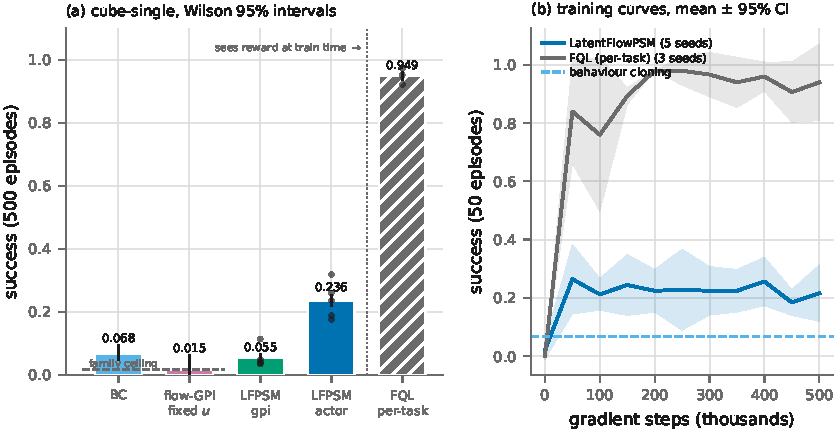
\includegraphics[width=0.9\linewidth]{figures/fig_actor_comparison.pdf}
\caption{Actor anatomy at the ceiling. Decoded actions recover 42\% of the local dataset action dispersion (63\% after a 100-step retrain), measured as per-dimension standard deviation against $k{=}32$ nearest-neighbor dataset actions at 64 states; the nearest decodable action to FQL's choice remains at 0.19 of mean action magnitude under one-step vs.\ full-ODE decoding and the retrain; scaling the latent prior raises coverage (0.63/0.99/1.41 at $1$/$1.5$/$2\times$) but moves that nearest decodable action \emph{away} from FQL's (0.19/0.23/0.28). With $Q$ varying by only 1.1\% of $|Q|$ over the latent prior, the actor's cloning term dominates and success saturates at 0.20--0.24 even for per-task latent RL.}
\label{fig:actor}
\end{figure}

\subsubsection*{Summary}
What we tried: restricting zero-shot RL to actions produced by a frozen behavior flow, with a successor measure over its latent space. What happened: a real improvement over imitation ($0.236$ vs.\ $0.068$ on cube), then a reproducible saturation near $0.22$. What we think is happening: the action restriction has two layers. The learned decoder covers substantially less local action variation than the data contains (42--63\%, i.e.\ 44--67\% relative to the estimator's split-half self-consistency reference of 0.936), and a strong per-task policy appears to exploit actions that are not represented in the local empirical action cloud at all ($0.577$ vs.\ $0.345$ normalized at matched candidate counts, $k=32$). The decoder-induced action interface is the leading explanation for the ceiling---rather than the successor measure, the task inference, or critic estimation---and the second layer raises the possibility that even a perfect behavior model would not lift it. Evidence: the indexed fixed-latent family contained almost no goal-reaching behaviors (0/233 reachability); per-task RL in the same latent space saturates at the same level as the zero-shot agent; decoded actions recover 42--63\% of local dataset dispersion and remain 0.19 (normalized) from a strong policy's choices under every decoding variant tried, while those choices are $1.64$--$1.80\times$ farther from the data's own nearest neighbors under candidate-count-matched statistics, robust across raw and standardized observation metrics and $k\in\{16,32,64\}$. What remains uncertain: how much actor optimization contributes on top of the coverage limit; and whether the interface limitation \emph{causally} determines the $0.22$ ceiling---the residual sweep is what can strengthen that claim. Next experiment: the residual-budget sweep, read in the three regimes above, which asks how much departure from the behavior data is needed to recover the forfeited performance.

\bibliography{references}
\bibliographystyle{iclr2027_conference}

\end{document}
